\documentclass[simple,14pt]{eskdtext}
\usepackage[T2A]{fontenc} % Поддержка русских букв
\usepackage[utf8]{inputenc} % Кодировка utf8
\usepackage[russian]{babel}

\usepackage{color}
\usepackage{xcolor}
\usepackage{cmap}
\usepackage{caption}
\usepackage{amsmath}
\usepackage{amstext}
\usepackage{amsfonts}
\usepackage{mathptmx}
\usepackage{listings}
\usepackage{geometry}
\geometry{left=2.5cm}
\geometry{right=1.0cm}
\geometry{top=2.0cm}
\geometry{bottom=2.0cm}

% Цвета для кода
\definecolor{string}{HTML}{B40000} % цвет строк в коде
\definecolor{comment}{HTML}{008000} % цвет комментариев в коде
\definecolor{keyword}{HTML}{1A00FF} % цвет ключевых слов в коде
\definecolor{morecomment}{HTML}{8000FF} % цвет include и других элементов в коде
\definecolor{сaptiontext}{HTML}{FFFFFF} % цвет текста заголовка в коде
\definecolor{сaptionbk}{HTML}{999999} % цвет фона заголовка в коде
\definecolor{bk}{HTML}{FFFFFF} % цвет фона в коде
\definecolor{frame}{HTML}{999999} % цвет рамки в коде
\definecolor{brackets}{HTML}{B40000} % цвет скобок в коде

% Настройки отображения кода
\lstset{
	language=C, % Язык кода по умолчанию
	morekeywords={*,...}, % если хотите добавить ключевые слова, то добавляйте
	% Цвета
	keywordstyle=\color{keyword}\ttfamily\bfseries,
	stringstyle=\color{string}\ttfamily,
	commentstyle=\color{comment}\ttfamily\itshape,
	morecomment=[l][\color{morecomment}]{\#}, 
	% Настройки отображения     
	breaklines=true, % Перенос длинных строк
	basicstyle=\ttfamily\footnotesize, % Шрифт для отображения кода
	backgroundcolor=\color{bk}, % Цвет фона кода
	%frame=lrb,xleftmargin=\fboxsep,xrightmargin=-\fboxsep, % Рамка, подогнанная к заголовку
	rulecolor=\color{frame}, % Цвет рамки
	tabsize=3, % Размер табуляции в пробелах
	% Настройка отображения номеров строк. Если не нужно, то удалите весь блок
	%numbers=left, % Слева отображаются номера строк
	stepnumber=1, % Каждую строку нумеровать
	numbersep=5pt, % Отступ от кода 
	numberstyle=\small\color{black}, % Стиль написания номеров строк
	% Для отображения русского языка
	extendedchars=true,
	literate={?}{{\"O}}1
	{?}{{\"A}}1
	{?}{{\"U}}1
	{?}{{\ss}}1
	{?}{{\"u}}1
	{?}{{\"a}}1
	{?}{{\"o}}1
	{~}{{\textasciitilde}}1
	{а}{{\selectfont\char224}}1
	{б}{{\selectfont\char225}}1
	{в}{{\selectfont\char226}}1
	{г}{{\selectfont\char227}}1
	{д}{{\selectfont\char228}}1
	{е}{{\selectfont\char229}}1
	{ё}{{\"e}}1
	{ж}{{\selectfont\char230}}1
	{з}{{\selectfont\char231}}1
	{и}{{\selectfont\char232}}1
	{й}{{\selectfont\char233}}1
	{к}{{\selectfont\char234}}1
	{л}{{\selectfont\char235}}1
	{м}{{\selectfont\char236}}1
	{н}{{\selectfont\char237}}1
	{о}{{\selectfont\char238}}1
	{п}{{\selectfont\char239}}1
	{р}{{\selectfont\char240}}1
	{с}{{\selectfont\char241}}1
	{т}{{\selectfont\char242}}1
	{у}{{\selectfont\char243}}1
	{ф}{{\selectfont\char244}}1
	{х}{{\selectfont\char245}}1
	{ц}{{\selectfont\char246}}1
	{ч}{{\selectfont\char247}}1
	{ш}{{\selectfont\char248}}1
	{щ}{{\selectfont\char249}}1
	{ъ}{{\selectfont\char250}}1
	{ы}{{\selectfont\char251}}1
	{ь}{{\selectfont\char252}}1
	{э}{{\selectfont\char253}}1
	{ю}{{\selectfont\char254}}1
	{я}{{\selectfont\char255}}1
	{А}{{\selectfont\char192}}1
	{Б}{{\selectfont\char193}}1
	{В}{{\selectfont\char194}}1
	{Г}{{\selectfont\char195}}1
	{Д}{{\selectfont\char196}}1
	{Е}{{\selectfont\char197}}1
	{Ё}{{\"E}}1
	{Ж}{{\selectfont\char198}}1
	{З}{{\selectfont\char199}}1
	{И}{{\selectfont\char200}}1
	{Й}{{\selectfont\char201}}1
	{К}{{\selectfont\char202}}1
	{Л}{{\selectfont\char203}}1
	{М}{{\selectfont\char204}}1
	{Н}{{\selectfont\char205}}1
	{О}{{\selectfont\char206}}1
	{П}{{\selectfont\char207}}1
	{Р}{{\selectfont\char208}}1
	{С}{{\selectfont\char209}}1
	{Т}{{\selectfont\char210}}1
	{У}{{\selectfont\char211}}1
	{Ф}{{\selectfont\char212}}1
	{Х}{{\selectfont\char213}}1
	{Ц}{{\selectfont\char214}}1
	{Ч}{{\selectfont\char215}}1
	{Ш}{{\selectfont\char216}}1
	{Щ}{{\selectfont\char217}}1
	{Ъ}{{\selectfont\char218}}1
	{Ы}{{\selectfont\char219}}1
	{Ь}{{\selectfont\char220}}1
	{Э}{{\selectfont\char221}}1
	{Ю}{{\selectfont\char222}}1
	{Я}{{\selectfont\char223}}1
	{і}{{\selectfont\char105}}1
	{ї}{{\selectfont\char168}}1
	{є}{{\selectfont\char185}}1
	{ґ}{{\selectfont\char160}}1
	{І}{{\selectfont\char73}}1
	{Ї}{{\selectfont\char136}}1
	{Є}{{\selectfont\char153}}1
	{Ґ}{{\selectfont\char128}}1
	{\{}{{{\color{brackets}\{}}}1 % Цвет скобок {
	{\}}{{{\color{brackets}\}}}}1 % Цвет скобок }
}

% Для настройки заголовка кода
\DeclareCaptionFont{white}{\color{сaptiontext}}
\DeclareCaptionFormat{listing}{\parbox{\linewidth}{\colorbox{сaptionbk}{\parbox{\linewidth}{#1#2#3}}\vskip-4pt}}
\captionsetup[lstlisting]{format=listing,labelfont=white,textfont=white}
\renewcommand{\lstlistingname}{Листинг} % Переименование Listings в нужное именование структуры
\renewcommand\contentsname{Оглавление}

%Section
\ESKDsectSkip{section}{12pt}{12pt}
%subsection
\ESKDsectSkip{subsection}{10pt}{10pt}
%subsubsection
\ESKDsectSkip{subsubsection}{8pt}{8pt}

%Грифт
%\renewcommand{\rmdefault}{ftm}

\setcounter{tocdepth}{2}

\ESKDdepartment{Министерство образования и науки Российской Федерации}
\ESKDcompany{Государственное общеобразовательное учреждение\\
	высшего профессионального образования\\
	Южно-Уральский государственный университет (НИУ)\\
	\begin{normalsize}\mbox{Факультет}~\mbox{«Компьютерные}~\mbox{технологии},~\mbox{управление}~и~\mbox{радиоэлектроника}~(ПС)»\\Кафедра «Системы управления»\end{normalsize}
	}
\ESKDauthor{Осипов~И.О.}
\ESKDchecker{\begin{scriptsize}Чернецкий В.О.\end{scriptsize}}
\ESKDnormContr{\begin{scriptsize}Чернецкий В.О.\end{scriptsize}}
\ESKDtitle{Семестровка по прикладной механике}
\ESKDtitleDesignedBy{Студент группы КТУР-334}{Осипов И.О.}
\ESKDtitleDesignedBy{Старший преподователь }{Чернецкий В.О.}
\ESKDtitle{Решение типовых задач на языке СИ}
\ESKDdocName{Пояснительная записка}
\ESKDsignature{КТУР--161101.2015.334.05 ПЗ}
\renewcommand{\ESKDtheTitleFieldX}{Челябинск 2015}
\renewcommand{\ESKDtheTitleFieldV}{к курсовой работе\\по дисциплине «Программирование на языках высокого уровня»}
\begin{document}
	\maketitle
	\section*{аннотация}
	\newpage
	\tableofcontents
	\newpage
	\section*{ВВЕДЕНИЕ}
	\addcontentsline{toc}{section}{ВВЕДЕНИЕ}
	\newpage
	\section[ПРОСТЫЕ ЗАДАЧИ]{ПРОСТЫЕ ЗАДАЧИ}
	
	\subsection{Задача 1}
	\subsubsection{Условие}
	Вычислить объем усеченного конуса по формуле $ V = \dfrac{h\pi}{3}(r_1^2+r_1 r_2 +r_1^2) $, где $ r_1, r_2$ -- радиусы оснований, а $h$ -- высота в см.
	\subsubsection{Формализация}
	Введем с клавиатуры геометрические размеры усеченного конуса: высоту $h$, радиусы верхнего и нижнего оснований $r_1$ и $r_2$. Если все параметры конуса неотрицательны, то можно вычислить объем конуса по формуле $ V = \dfrac{h\pi}{3}(r_1^2+r_1 r_2 +r_1^2) $. В случае, если хотя бы один параметр конуса меньше 0, то такой конус не существует и нужно вывести ошибку и завершить программу.
	\subsubsection{Блок схема}
	Блок схема программы, описанной в предыдущем пункте представлена на рисунке \ref{fig:block1}.
\begin{figure}[h!]
\centering
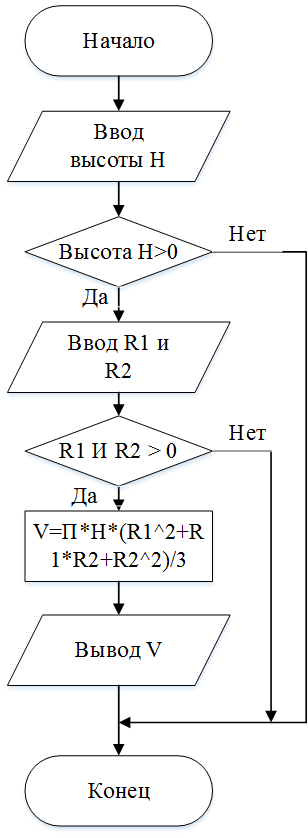
\includegraphics[width=0.222\linewidth]{./task_1/block1}
\caption{Блок-схема задачи 1}
\label{fig:block1}
\end{figure}

	\subsubsection{Код программы}
	\begin{lstlisting}[label=some-code1,caption=Задача 1]
/// Вычислить объем усеченного конуса по формуле
#include <stdio.h>
#include <stdlib.h>
#include <math.h>
		
int main()	{
   double h, r1, r2;
   printf("input height ");
   scanf("%lf",&h);
   if (h < 0) { // Проверка положительности высоты конуса
      printf("Error: h=0");
	  return 0;
   }
  
   printf("input radiuses ");
   scanf("%lf %lf",&r1, &r2);
		
   if ((r1 < 0)||(r2 < 0)) {// Проверка положительности радиусов оснований конуса
      printf("Error: radius < 0");
      return 0;
   }
		
   printf("volume of com is %f ", h * M_PI * (r1 * r1 + r1 * r2 + r2 * r2) / 3.);
   getch();
   return 0;
}
	\end{lstlisting}
	\subsubsection{Результат работы программы}
	Результат работы программы представлен на рисунке \ref{fig:result1}.
	\begin{figure}
\centering
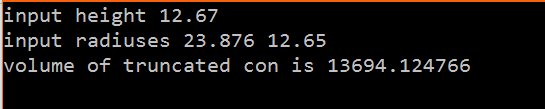
\includegraphics[width=0.7\linewidth]{task_1/result1}
\caption{Окно и результат работы программы 1}
\label{fig:result1}
\end{figure}

	\subsubsection{Инструкция пользователя}
	Для запуска программы необходимо запустить исполняемый файл task1.exe из папки проекта и следуя инструкциям на экране ввести данные, после этого программа выведет результат расчета. 
	   
	\subsection{Задача 2}
	\subsubsection{Условие}
	Вычислить $ x=\left(\frac{(a+b)^{2}c}{m-n}\right)^2 $.
	\subsubsection{Формализация}
	После ввода с клавиатуры операндов формулы $ a,b,c,m,n $ и проверки неравенства $0$ знаменателя, можно вычислить формулу $ x=\left( \frac{(a+b)^{2}}{m-n}\right)^2 $ и вывести результат на экран.Если знаменатель равен $0$, то следует вывести ошибку и завершить работу. 
	\subsubsection{Блок схема}
	Блок-схема программы, описанной выше представлена на рисунке \ref{fig:block2}.
	 \begin{figure}[h!]
\centering
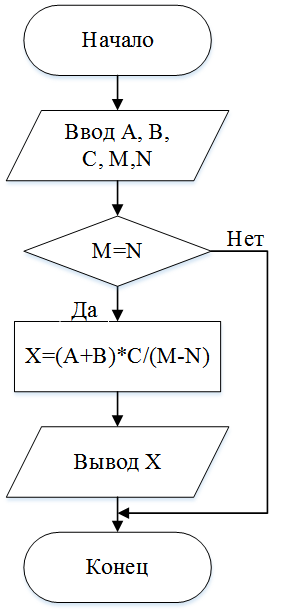
\includegraphics[width=0.25\linewidth]{task_2/block2}
\caption{Блок-схема задачи 2}
\label{fig:block2}
\end{figure}

	\subsubsection{Код программы}
	\begin{lstlisting}[label=some-code2,caption=Задача 2]
	/**
		вычислить формулу x=(((a+b)*c)/(m-n))^2
	**/
	#include <stdio.h>
	#include <stdlib.h>
		
	int main()
	{
	double a,b,c,m,n;
		
	double x;
		
	printf("input a ");
	scanf("%lf",&a);
		
	printf("input b ");
	scanf("%lf",&b);
		
	printf("input c ");
	scanf("%lf",&c);
		
	printf("input m ");
	scanf("%lf",&n);
		
	printf("input n ");
	scanf("%lf",&n);
	
	if (m != n) { //Проверка для исключения деления на 0
	x = ((a + b) * c) / (m - n);
	printf("x is %f", x * x);
	}
	else printf("error: m = n!!!");
	
	return 0;
	}
	\end{lstlisting}
	\subsubsection{Результат работы программы}
	Результат работы программы представлен на рисунке
	\subsubsection{Инструкция пользователя}
	
	\subsection{Задача 3}
	\subsubsection{Условие}
	Найти все пары двузначных натуральных чисел, таких, что значение произведения чисел не меняется, если поменять местами цифры каждого из сомножителей. 
	\subsubsection{Формализация}
	Для нахождения всех таких чисел будем перебирать каждый из множителей от 10 до 99. Для каждого варианта каждого изз множителей, сдлаем его копию, с измененным порядком цифр. Затем сравним произведение полученных копий с произведением исходных множителей. Если произведения равны, то выведем пару множителей на экран.
	\subsubsection{Блок схема}
	\subsubsection{Код программы}
	\begin{lstlisting}[label=some-code3,caption=Задача 3]
	/**
	* Найти все пары двухзначных натуральных чисел, таких,
	* что значение произведенения чисел не изменится, если поменять местами
	* цифры каждого из сомножителей
	*/
	#include <stdio.h>
	#include <stdlib.h>
	
	int main()
	{
	int a,b,ka,kb;
	for (a = 10;a < 100; a++)
	for (b = 10; b < 100; b++) {
	ka = (a / 10) + 10 * (a % 10);
	kb = (b / 10) + 10 * (b % 10);
	if (ka * ka == a * b) printf("%d %d \n", a, b);
	}
	return 0;
	}
	\end{lstlisting}
	\subsubsection{Результат работы программы}
	Результат работы программы представлен на рисунке 
	\subsubsection{Инструкция пользователя}
	
	\subsection{Задача 4}
	\subsubsection{Условие}
	Протабулировать функцию $ y=\frac{\sin(x)+\cos^2(x)}{\sin(x^2)-3\tg(\frac{x}{5})} $ на интервале $ 2\leq x\leq11 $ с шагом $h=1$.
	\subsubsection{Формализация}
	
	\subsubsection{Блок схема}
	\subsubsection{Код программы}
	\begin{lstlisting}[label=some-code3,caption=Задача 4]
	/**
	*
	* Протабулировать функцию
	* y=(sin(x)+cos^2(x))/(sin(x^2)-3*tan(x/5));
	* на интервале 2..11 с шагом 1.
	*/
	#include <stdio.h>
	#include <stdlib.h>
	#include <math.h>
	
	double f(double x) {
	return (sin(x) + cos(x) * cos(x)) / (sin(x * x) - 3. * tan( x / 5.));
	}
	
	int main()	{
	   int i;
	   for (i = 2; i < 12; i++)
	   printf("y(%d) = %f \n", i, f(i));
	   return 0;
	}
	\end{lstlisting}
	\subsubsection{Результат работы программы}
	Результат работы программы представлен на рисунке 
	\subsubsection{Инструкция пользователя}
	
	\subsection{Задача 5}
	\subsubsection{Условие}
	\subsubsection{Формализация}
	\subsubsection{Блок схема}
	\subsubsection{Код программы}
	\begin{lstlisting}[label=some-code3,caption=Задача 5]
	/**
	*
	* Протабулировать функцию
	* y=(sin(x)+cos^2(x))/(sin(x^2)-3*tan(x/5));
	* на интервале 2..11 с шагом 1.
	*/
	#include <stdio.h>
	#include <stdlib.h>
	#include <math.h>
	
	double f(double x) {
	return (sin(x) + cos(x) * cos(x)) / (sin(x * x) - 3. * tan( x / 5.));
	}
	
	int main()	{
	   int i;
	   for (i = 2; i < 12; i++)
	      printf("y(%d) = %f \n", i, f(i));
	   return 0;
	}
	\end{lstlisting}
	\subsubsection{Результат работы программы}
	\subsubsection{Инструкция пользователя}
	
	\subsection{Задача 6}
	\subsubsection{Условие}
	\subsubsection{Формализация}
	\subsubsection{Блок схема}
	\subsubsection{Код программы}
	\begin{lstlisting}[label=some-code3,caption=Задача 3]
	/**
	* Найти все пары двухзначных натуральных чисел, таких,
	* что значение произведенения чисел не изменится, если поменять местами
	* цифры каждого из сомножителей
	*/
	#include <stdio.h>
	#include <stdlib.h>
	
	int main()
	{
	int a,b,ka,kb;
	for (a = 10;a < 100; a++)
	for (b = 10; b < 100; b++) {
	ka = (a / 10) + 10 * (a % 10);
	kb = (b / 10) + 10 * (b % 10);
	if (ka * ka == a * b) printf("%d %d \n", a, b);
	}
	return 0;
	}
	\end{lstlisting}
	\subsubsection{Результат работы программы}
	\subsubsection{Инструкция пользователя}
	
	\subsection{Задача 7}
	\subsubsection{Условие}
	\subsubsection{Формализация}
	\subsubsection{Блок схема}
	\subsubsection{Код программы}
	\begin{lstlisting}[label=some-code3,caption=Задача 3]
	/**
	* Найти все пары двухзначных натуральных чисел, таких,
	* что значение произведенения чисел не изменится, если поменять местами
	* цифры каждого из сомножителей
	*/
	#include <stdio.h>
	#include <stdlib.h>
	
	int main()
	{
	int a,b,ka,kb;
	for (a = 10;a < 100; a++)
	for (b = 10; b < 100; b++) {
	ka = (a / 10) + 10 * (a % 10);
	kb = (b / 10) + 10 * (b % 10);
	if (ka * ka == a * b) printf("%d %d \n", a, b);
	}
	return 0;
	}
	\end{lstlisting}
	\subsubsection{Результат работы программы}
	\subsubsection{Инструкция пользователя}
	
	\newpage
	\section[СЛОЖНАЯ ЗАДАЧА]{сложная задача}
	\subsection{Условие}
	Обратить заданную матрицу методом окаймления. Результат обращения проверить на корректность, умножив на заданную матрицу. 
	\subsection{Формализация}
	
	\subsection{Блок схема}
	\subsection{Код программы}
	\subsection{Результат работы программы}
	\subsection{Инструкция пользователя}
	
	\section*{заключение}
	\addcontentsline{toc}{section}{ЗАКЛЮЧЕНИЕ}
	\section*{список  литературы}
	\addcontentsline{toc}{section}{СПИСОК ЛИТЕРАТУРЫ}
\end{document}